\documentclass[a4paper]{article}
%\setbeameroption{show notes on second screen=right} % Both
% Theme choice:
\usepackage{geometry}
\geometry{
	a4paper,
	total={170mm,257mm},
	left=20mm,
	top=20mm,
}
\usepackage{tikz-feynman}
\usepackage{animate}
\usepackage{amsmath}
\usepackage{cancel}
\usepackage{multicol}
\usepackage{physics}
\usepackage{graphicx}
\usepackage{amsfonts}
\usepackage{caption}
\usepackage{wrapfig}
\usepackage{pgfplots}
\usepackage{subfigure}
\usepackage{listings}
\pgfplotsset{compat=1.15}
\captionsetup{singlelinecheck=false}
\usepackage[backend=bibtex,bibencoding=utf8,doi=false,isbn=false,url=false,eprint=false,indexing=false,style=authoryear]{biblatex}
\addbibresource{library}
\AtEveryBibitem{%
	\clearname{translator}%
	\clearlist{publisher}%
	\clearfield{pagetotal}%
}
\usepackage{MnSymbol,wasysym}
\usepackage[toc,page]{appendix}
\usetikzlibrary{snakes}
\usetikzlibrary{shapes.geometric, calc}
\author{Vo Chau Duc Phuong}
% Title page details: 
\title{Simulation of Liquid Argon}
\begin{document}
	\maketitle
\tableofcontents
\section{Initial}
\quad Using the FORTRAN, I simulate the liquid Argon in the Lennard-Jones potential between the particles. The input value into the code will be these parameters and variables:\\
\rule{\textwidth}{1pt}
{\small
 \begin{lstlisting}
integer :: n = 864, bc = 1, tr = 0 !bc: periodic boundary, tr: poor-mans algorithm
real, allocatable :: dens(:,:,:)
!crucial parameters
real, parameter :: T = 94.4, kb= 1.380649*10.**(-16.)
real, parameter :: m = 39.95*1.67*10.**(-24), sigma = 3.4*10**(-8.)
real, parameter :: ep = 120.*kb, rc = 2.25, L = 10.229, halfL = 10.229/2.
!time parameters
integer :: nt, ntrelax
real, parameter :: tmin = 0.0, tmax = 100.0, trelax = 10.0 !in ps
real ::  dt = 0.01  !ps
\end{lstlisting}}
\rule{\textwidth}{1pt}\null\vspace{0.5cm}
\normalsize\null
\quad The first line is specify the number of particles, use the parameter and poor-mans thermal-stat or not. (in this case, no thermal-stats).\\\null
\quad Second line is the define of the density matrix, contains the position and velocity of all particles.\\\null
\quad Crucial parameter will be in the unit of cgs. The time parameters as shown.\\
\rule{\textwidth}{1pt}
{\small
\begin{lstlisting}
subroutine Initial()
implicit none
integer :: i, j, k, p
real :: spacing, v_stddev, rand1, rand2, Tp, E
allocate(dens(n,3,2))
ntrelax = int(trelax/dt); nt = int((tmax - tmin)/dt)
dt = dt*1.0e-12*(ep/m)**0.5*1./sigma
! Initialize densitions randomly within the box
spacing = L / (int(n**(1.0/3.0)) + 1) ! Adjust spacing to avoid boundary
p = 0
do i = 0, int(n**(1.0/3.0))
do j = 0, int(n**(1.0/3.0))
do k = 0, int(n**(1.0/3.0))
p = p + 1
if (p > n) exit
dens(p,1,1) = i * spacing
dens(p,2,1) = j * spacing
dens(p,3,1) = k * spacing
end do
if (p > n) exit
end do
if (p > n) exit
end do
v_stddev = sqrt(kb * T / m)
do i = 1, n
do j = 1, 3
call random_number(rand1); call random_number(rand2)
dens(i,j,2) = v_stddev * sqrt(-2.0 * log(rand1)) &
* cos(2.0 * 3.14159265359 * rand2)
end do
end do
do i = 1, 3
dens(:,i,2) = dens(:,i,2) - sum(dens(:,i,2))/n
end do
Tp = sum(dens(:,:,2)**2.) * m / (3.0 * n * kb)
dens(:,:,2) = dens(:,:,2) * sqrt(T / Tp)
dens(:,:,2) = dens(:,:,2) / (ep/m)**0.5 ! Convert to dimensionless units
end subroutine
\end{lstlisting}}
\rule{\textwidth}{1pt}\\\null
\quad First, I generate the position of the particles in a lattice to avoid the very strong at the near interaction of Leornard-Johnes potential and also generate the velocity in each direction arcording the Boltzmann distribution using random-number generator.
\begin{figure}[h]
\begin{center}
	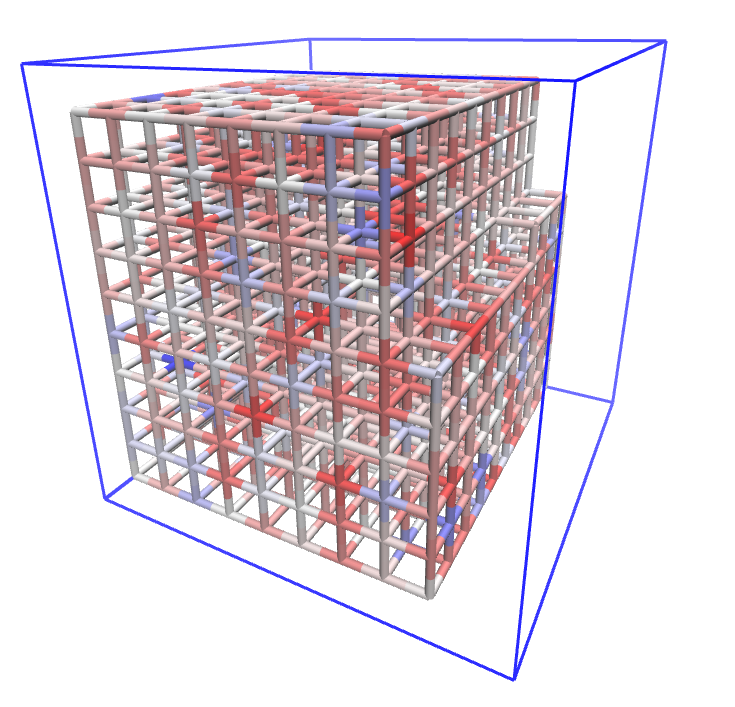
\includegraphics[width = 0.5\linewidth]{Images/Lattice.png}
\caption{Initial position of atoms and their colored according to their initial velocity}
\end{center}
Then, using the do loop, delete the net-momentum velocity. After all, scale every thing to our desire temperature using the relation: \(v \sim \sqrt{T}\) and converge to the dimensionless unit (which position is already in). According to the paper, the unit of length is \(\sigma\), the unit of velocity is \(\sqrt{\epsilon/m}\) and the unit of time is \(10^{-12}*(\epsilon/m)^{1/2}(1/\sigma)\) (the line with \(dt = dt...\)) to match which the rest.
\end{figure}
\section{Method}
To begin with our simulation, I need to deal with the acceleration of the particle each time, which will be calculated according to:
\begin{equation}
\dv{v_i}{t} = a_i = 24 \frac{\epsilon}{m} \sum_{j \neq i} \frac{x_i - x_j}{r_{ij}^2} \bigg( 2 \bigg(\frac{\sigma}{r_{ij}}\bigg)^{12} - \bigg(\frac{\sigma}{r_{ij}}\bigg)^{6}\bigg)
\end{equation}
or in the unitless dimension:
\begin{equation}
	\dv{v_i}{t} = a_i = 24 \sum_{j \neq i} \frac{x_i - x_j}{r_{ij}^2} \bigg( \bigg(\frac{2}{r_{ij}}\bigg)^{12} - \bigg(\frac{1}{r_{ij}}\bigg)^{6}\bigg)
\end{equation}
which save a lot of calculation resource, along with the minimal image technique, as shown in the code:
\rule{\textwidth}{1pt}{\small
\begin{lstlisting}
subroutine calaccf(acc, dens)
implicit none
integer :: i, j, k
real :: rr, rri, rri2, rri6, dr(3), coef(3)
real, intent(out) :: acc(n,3)
real, intent(in) :: dens(n,3)
acc = 0.0
do i = 1, n
do j = i + 1, n
dr(:) = dens(i,:) - dens(j,:)
if (dr(1) >  halfL)  dr(1) = dr(1) - L
if (dr(1) < -halfL)  dr(1) = dr(1) + L
if (dr(2) >  halfL)  dr(2) = dr(2) - L
if (dr(2) < -halfL)  dr(2) = dr(2) + L
if (dr(3) >  halfL)  dr(3) = dr(3) - L
if (dr(3) < -halfL)  dr(3) = dr(3) + L
rr = sum(dr**2)
if (rr < rc**2.) then
rri2 = 1.0 / rr; rri6 = rri2 * rri2 * rri2
coef = rri2 * (2.0 * rri6 * rri6 - rri6)
acc(i,:) = acc(i,:) + coef*dr(:)
acc(j,:) = acc(j,:) - coef*dr(:)
end if
end do
end do
acc = acc*24.0
end subroutine
\end{lstlisting}}

\rule{\textwidth}{1pt}
This return the acceleration that will be used in the velocity Verlet algorithm:

\rule{\textwidth}{1pt}
{\small
\begin{lstlisting}
subroutine verlexp()
implicit none
integer :: i, j
real :: acc(n,3), temp(n,3,2), Tp, vhalf(n,3)
call calaccf(acc, dens(:,:,1))
!print*, maxval(acc), minval(acc)
!$OMP PARALLEL DO PRIVATE(i,j) SCHEDULE(dynamic)
do i = 1, n
do j = 1, 3
vhalf(i,j) = dens(i,j,2) + 0.5 * dt * acc(i,j)
dens(i,j,1) = dens(i,j,1) + dt * vhalf(i,j)
end do
end do
!$OMP END PARALLEL DO
call calaccf(acc, dens(:,:,1))
!$OMP PARALLEL DO PRIVATE(i,j) SCHEDULE(dynamic)
do i = 1, n
do j = 1, 3
dens(i,j,2) = vhalf(i,j) + 0.5 * dt * acc(i,j)
end do
end do
!$OMP END PARALLEL DO
! Apply periodic boundary conditions
do i = 1, n
do j = 1, 3
dens(i,j,1) = mod(dens(i,j,1), L)
if (dens(i,j,1) < 0.) dens(i,j,1) = dens(i,j,1) + L
end do
end do
if ((abs(Tp - T) > 5) .AND. (tr == 1)) then
Tp = sum(dens(:,:,2)**2.) * m / (3. * kb * n) * (ep / m) ! Temperature in Kelvin
!$OMP PARALLEL DO PRIVATE(i,j) SCHEDULE(dynamic)
do i = 1, n
do j = 1, 3
dens(i,j,2) = dens(i,j,2) * sqrt(T / Tp)
end do
end do
!$OMP END PARALLEL DO
end if
end subroutine
\end{lstlisting}}
\rule{\textwidth}{1pt}
This althogithm is used more commonly than the basic Verlet, but with the same error. The standard sudo-code is:
\begin{itemize}
\item Calculate \(v(t + \frac{1}{2} \Delta t)  = v(t)  + \frac{1}{2} a(t)\Delta t\)
\item Calculate \(x(t + \Delta t) = x(t) + v(t + \frac{1}{2} \Delta t) \Delta t\)
\item Derive \(a(t+ \Delta t)\) from \(x(t + \Delta t) \)
\item Calculate \(v(t + \Delta t) = v(t + \frac{1}{2} \Delta t) + \frac{1}{2} a ( t+ \Delta t) \Delta t\)
\end{itemize}
\quad After calculate the position, I will using the periodic boundary condition as shown to put the particle to the other side of the box in case that they moved out of it in the last calculation.\\ \null
\quad In these calculation, to reduce the time-cost, I using the library openmp multiple times to run in parallel the process and also to avoid the overlap of step in the sudo-code above.\\\null
The whole system will be putted in the relaxation phase before being recorded into the lammpstrj format:

\rule{\textwidth}{1pt}
\begin{lstlisting}
ITEM: TIMESTEP
0
ITEM: NUMBER OF ATOMS
864
ITEM: BOX BOUNDS pp pp pp
0.00000000       10.2290001    
0.00000000       10.2290001    
0.00000000       10.2290001    
ITEM: ATOMS id x y z vx vy vz
1 9.08721542 8.11245155 9.03801727 -1.09344363 0.618355691 0.164400533    
2 9.73000050 9.10251331 1.50361073 1.60687697 0.147791833 0.713256001 
\end{lstlisting}

\rule{\textwidth}{1pt}
The program will be:

\rule{\textwidth}{1pt}
\begin{lstlisting}
program main
use liquid
implicit none
integer :: it
real :: Tp, tcurrent
call initial()
call writeinitial()
do it = 0, ntrelax
if (mod(it, 100) == 0) then
print*, "Current time: ", it*dt*1e12*(m/ep)**0.5*sigma
print*, "Temperature: ", sum(dens(:,:,2)**2.) * m / (3.0 * n * kb) * (ep / m)
end if
call verlexp()
end do
print*, "Relaxation finished"
Tp = sum(dens(:,:,2)**2.) * m / (3.0 * n * kb) * (ep / m)
dens(:,:,2) = dens(:,:,2) * sqrt(T / Tp)
do it = 0, nt
if (mod(it, 100) == 0) then
print *, "Current time: ", it*dt*1e12*(m/ep)**0.5*sigma
print *, "Temperature: ", sum(dens(:,:,2)**2.) * m / (3.0 * n * kb) * (ep / m)
end if
tcurrent = tmin + it*dt*1e12*(m/ep)**0.5*sigma
if (mod(it, 10) == 0.) then
call writetraject(it)
call write_energy(it)
end if
call verlexp()
end do
deallocate(dens)
end program
\end{lstlisting}
\rule{\textwidth}{1pt}
After the relaxation, all the velocity will be shifted to the desired temperature however using the poor-mans or not before being recorded into the file.
\section{Results and Discussion}
Using the parameter from the beginning, the simulation show some interesting properties:

\end{document}